% this file is called up by thesis.tex
% content in this file will be fed into the main document

%: ----------------------- name of chapter  -------------------------
\chapter{Problem Statement} % top level followed by section, subsection

%: ----------------------- paths to graphics ------------------------

% change according to folder and file names
\ifpdf
    \graphicspath{{X/figures/PNG/}{X/figures/PDF/}{X/figures/}}
\else
    \graphicspath{{X/figures/EPS/}{X/figures/}}
\fi

%: ----------------------- Mobile Cloud Middleware ------------------------

In this chapter, the prototype developed in Context Sensor Data on Demand
for Mobile Users Supported by XMPP \cite{prev_thesis} is described. The prototype was successful, but had some downsides. Secondly, an overview of the problems with the existing implementation is given. 
\todo{Add a small introduction of who wrote the previous thesis etc}

\section{Current Solution}

The current solution \cite{prev_thesis} has three main components:
\begin{enumerate}
\item Arduino sensor module
\item OpenFire XMPP server
\item Data collection server in the cloud (referred to as the server from here on)
\end{enumerate}

There were two separate configurations described in Context Sensor Data on Demand
for Mobile Users Supported by XMPP - one using Wi-Fi and the other Ethernet for network communication. Only Wi-Fi configuration is considered in this thesis due to the fact that the availability of an Ethernet connection (a cable) usually means that there is a power outlet nearby. 

\subsection{Arduino}

The first component is the Arduino sensor module. The hardware configuration is based on the Arduino Mega ADK board. Wireless Shield with RN-XV WiFly module is mounted on top of the board. Wireless Shield and Arduino board communicate over UART (hardware serial). TinkerKit Mega Sensor Shield is mounted on top of the Wireless Shield with 7 modules attached to it: 4 LED indicator lights, Hall, thermistor and LDR sensors. The external power source used is a 9V battery.

On the software side, the implementation mainly relies on a XMPP library and WiFly module library called WiFlyHQ. The WiFlyHQ library is responsible for creating a TCP connection and communication over the network, the XMPP library handles all the XMPP implementation details. 

The sketch itself is fairly straightforward - in $setup()$ a wireless network is joined, a TCP connection established and lastly a XMPP session is initialized. In $loop()$ all connections are checked and reestablished if needed. Then the last transmit time variable is compared to the current time and if the report step amount (currently 10 seconds) has passed, data is collected from the sensors, formatted to appropriate JSON string and sent to the server-side client. 

\subsection{XMPP Communication}

Both the data collection server and Arduino module are XMPP clients. The XMPP OpenFire server runs in the cloud and provides XMPP communications to both clients. Clients connect to the same chat where the server listens for messages from the sensor module. When a message is received by the server, sensor data is parsed from it and saved in a database.

\todo{xmpp initialization time}
XMPP session lifecycle can be seen in \autoref{xmpp_lifecycle}. With the current implementation, steps 1 - 5 are done once when establishing the connection or when the connection drops. Data transmission step is done every 10 seconds and the last 2 steps are done when the connection is closed.

\begin{figure}[H]
\centering
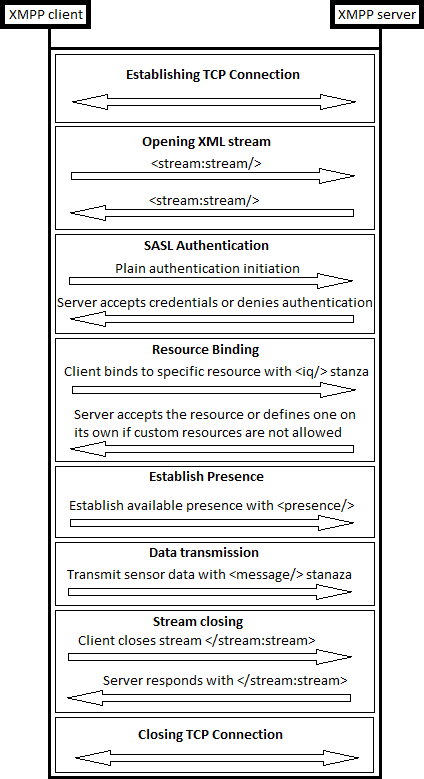
\includegraphics[scale=0.6]{3/figures/xmpp_session.png}
\caption{XMPP Session Lifecycle}
\label{xmpp_lifecycle}
\end{figure}

\subsection{Data Collection Server}
The data collection server is responsible for gathering sensor data and saving it in a database. Its implementation is written in Java and uses Smack XMPP API to communicate over XMPP. Data is stored in a H2 database, because of its simplicity and suitability for prototyping. 

The database has three main tables - sensors, data and locations. Locations table has different sensor module locations, sensors table has different types of sensors and data has data gathered from different locations and sensors. The data model can be seen in \autoref{data_model_initial}.

\begin{figure}[H]
\centering
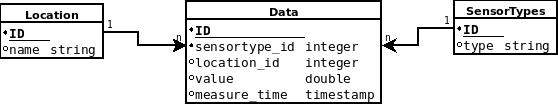
\includegraphics[scale=0.6]{3/figures/data_model_initial.jpg}
\caption{Server-side Data Model}
\label{data_model_initial}
\end{figure}

\section{Problems}

Previously mentioned implementation has a few problems which will be discussed in this section. The two main points are power consumption and data collection flexibility. 

According to the tests run in the previous thesis, the battery is able to power the module for 161,5 minutes using Wi-Fi. \cite[p. 50-51]{prev_thesis} This, however, is not sufficient to enable actual data collection from a remote location. The problem can be addressed by using a larger battery, but the actual power consumption should be optimized, too. Additionally, the 10 second data transmission interval is hard coded into the Arduino sensor module, which does not provide enough flexibility. The following chapter described changes to the hardware, software and communication methods which improve on these error points.

\subsection{Hardware}

The hardware configuration has two main problems. Firstly, communication over the wireless module can be unstable at times, because parts of the messages might be missing or scrambled when read from the UART \cite[p. 47]{prev_thesis}. Since XMPP session initialization is quite verbose, the possibility of receiving scrambled or incomplete messages effects the process. 

Secondly, all parts of the hardware configuration are run in full power mode. As there is a 10 second gap between data transmission and sensor reads, there is a time period when most components are idling. This, in turn, means that some parts of hardware could use less power during these intervals and therefore reduce overall power consumption.

\subsection{Software}

With the existing implementation $loop()$ is called consecutively and time differences are checked to determine when 10 seconds has passed using the internal $millis()$ function, which gives the current Unix time. Since we have a 10 second interval, we do not need to waste cycles on time difference checks we now will fail for the next 10 seconds. A way to delay program execution could be used to stop the execution until we know the defined amount of time has passed. 

In addition, as messages from the Wireless Shield might not be complete and  XMPP session initialization is a verbose process, the current XMPP implementation hangs when scrambled messages are received during session start up. The library checks from complete XML tags, but when the attributes are incomplete, connection will not be successful and the session initialization code hangs.

\subsection{Power Consumption}

Power consumption is the main problem this thesis focuses on. As a 9V battery has an average capacity of 400 $mAh$ at 100 $mA$ current, the resource is quite limited. With the existing configuration, the average current drawn is 108 $mA$. Battery lifetime tests in the previous thesis showed that the module runs for 161,5 minutes on a 9V battery \cite[p. 50]{prev_thesis}. However, 161,5 minutes is not enough to gather contextual data for the proposed data collection system. The batteries need to be changed too often for it to be a viable solution. 
\todo{how should i reference all the data collected?}


% ---------------------------------------------------------------------------
%: ----------------------- end of thesis sub-document ------------------------
% ---------------------------------------------------------------------------

